\subsection{Datasets}
\label{sec:datasets}
{\bf Write a more in depth discussion of the datasets and the  experiments. }
We used the following two datasets in our experiments: (1) Interesting iPhone cases:
for generating the ground truth data we hired workers from {\em Amazon Mechanical Turk (AMT)} to label a collection
of nearly 20,000 iPhone cases on {\em eBay}. The details of this step is beyond the scope of this paper, however we used insights from
interesting iPhone cases found on {\em Pinterest} and {\em eBay's} user behavior data in order to generate a balanced data-set. 
We then pulled our final dataset from the annotated by selecting only those instances where the annotators all labeled it as
positive (i.e., interesting) or negative (i.e., uninteresting). The final data-set consists of 2179 positive and 9770 negative instances for
a total of 11,949 instances. For each instance, the product title of
the corresponding {\em eBay} listing was used as the input. In this case we are
dealing with very short text snippets, usually 10 to 12 words each. To
train a topic model, we used a larger, more broader set of about
2 million product titles, grouped based on {\em eBay} categorical information into about 8,000
documents of approximately 200 titles each; (2) {\em NSF}
abstracts: for the second dataset we used a set of 61,902 National Science Foundation
Scholarship proposal abstracts (see~\cite{bache:2013} for more details) to evaluate how our diversity measure
compares to other methods on larger pieces of text. We used this set
for training a topic model, however to get labeled data, we had to
generate artificial examples, by randomly mixing pairs of abstracts that we
could expect to be either similar (small diversity) or very different
(high diversity) and labeling them accordingly. We generated 5,000 of
those examples with positive and negative labels evenly represented. For both datasets, we used the Mallet LDA implementation and learned a separate topic model with $400$ topics.

\subsection{Baselines}
\label{sec:baselines}
{\bf More information about the baselines. Particularly, the entropy
  with topic similarity is essentially also a new approach and works
  well. 

Add the DPP baseline (expected sample size, because detereminant is
unstable). Discussion probably
should include the fact that it is correlated with the document
length, which has more impact with eBay dataset. Include plots of ROC
curves with them.

More info about the auto-encoders and word2vec method.}

We present two sets of results. First, we present
ROC curves comparing different measures of topic diversity in an unsupervised setting 
(labeled data is only used for generating the curves). 
Figures~\ref{fig:phonecases-comparison} and \ref{fig:nsf-comparison}
compare our diversity metric using both topic similarity and context
conditioning (labeled by {\em JSD-Sim-Con}) with a few baselines;
namely LDA topic entropy, LDA topic entropy using topic similarity
(labeled by {\em Entropy-Sim}), {\em Rao diversity} and a measure
based on Determinantal Point Processes. The entropy has
been previously tested as a measure of document diversity with quite
underwhelming results in \cite{bache:2013}, where the authors proposed 
Rao diversity as a solution, which incorporates the topic similarity
information to provide better accuracy. We asked the question whether
the poor performance of entropy might be due to an suboptimal choice of
topic distribution, which led to our topic similarity
transformation. This technique can be used on any topic distribution
by simply multiplying it by the topic similarity matrix, and then
renormalizing. We present the performance of entropy with the topic
similarity transformation to verify that this approach improves the results not
only for Jensen-Shannon Divergence, but for other measures as well.

Determinantal Point Processes (DPP) have recently gained popularity as a
useful tool for diverse sampling, with many applications {\bf citation
  needed}. We were interested to see if they can also be useful for
measuring the diversity of a set provided as input. Given a set of
instances described as feature vectors $U=\{v_i\}_{i=1}^N\subset \rr^T$, DPP defines a
sampling model for selecting a subset of $S=\{v_{i_j}\}_{j=1}^k$, by
setting the probability of $S$ to be the determinant of the Gram
matrix corresponding to those vectors: $P(S) = \det (S^T S)$.
% \begin{figure}
%         \centering
%         \begin{subfigure}[b]{0.24\textwidth}
%                 \centering
%                 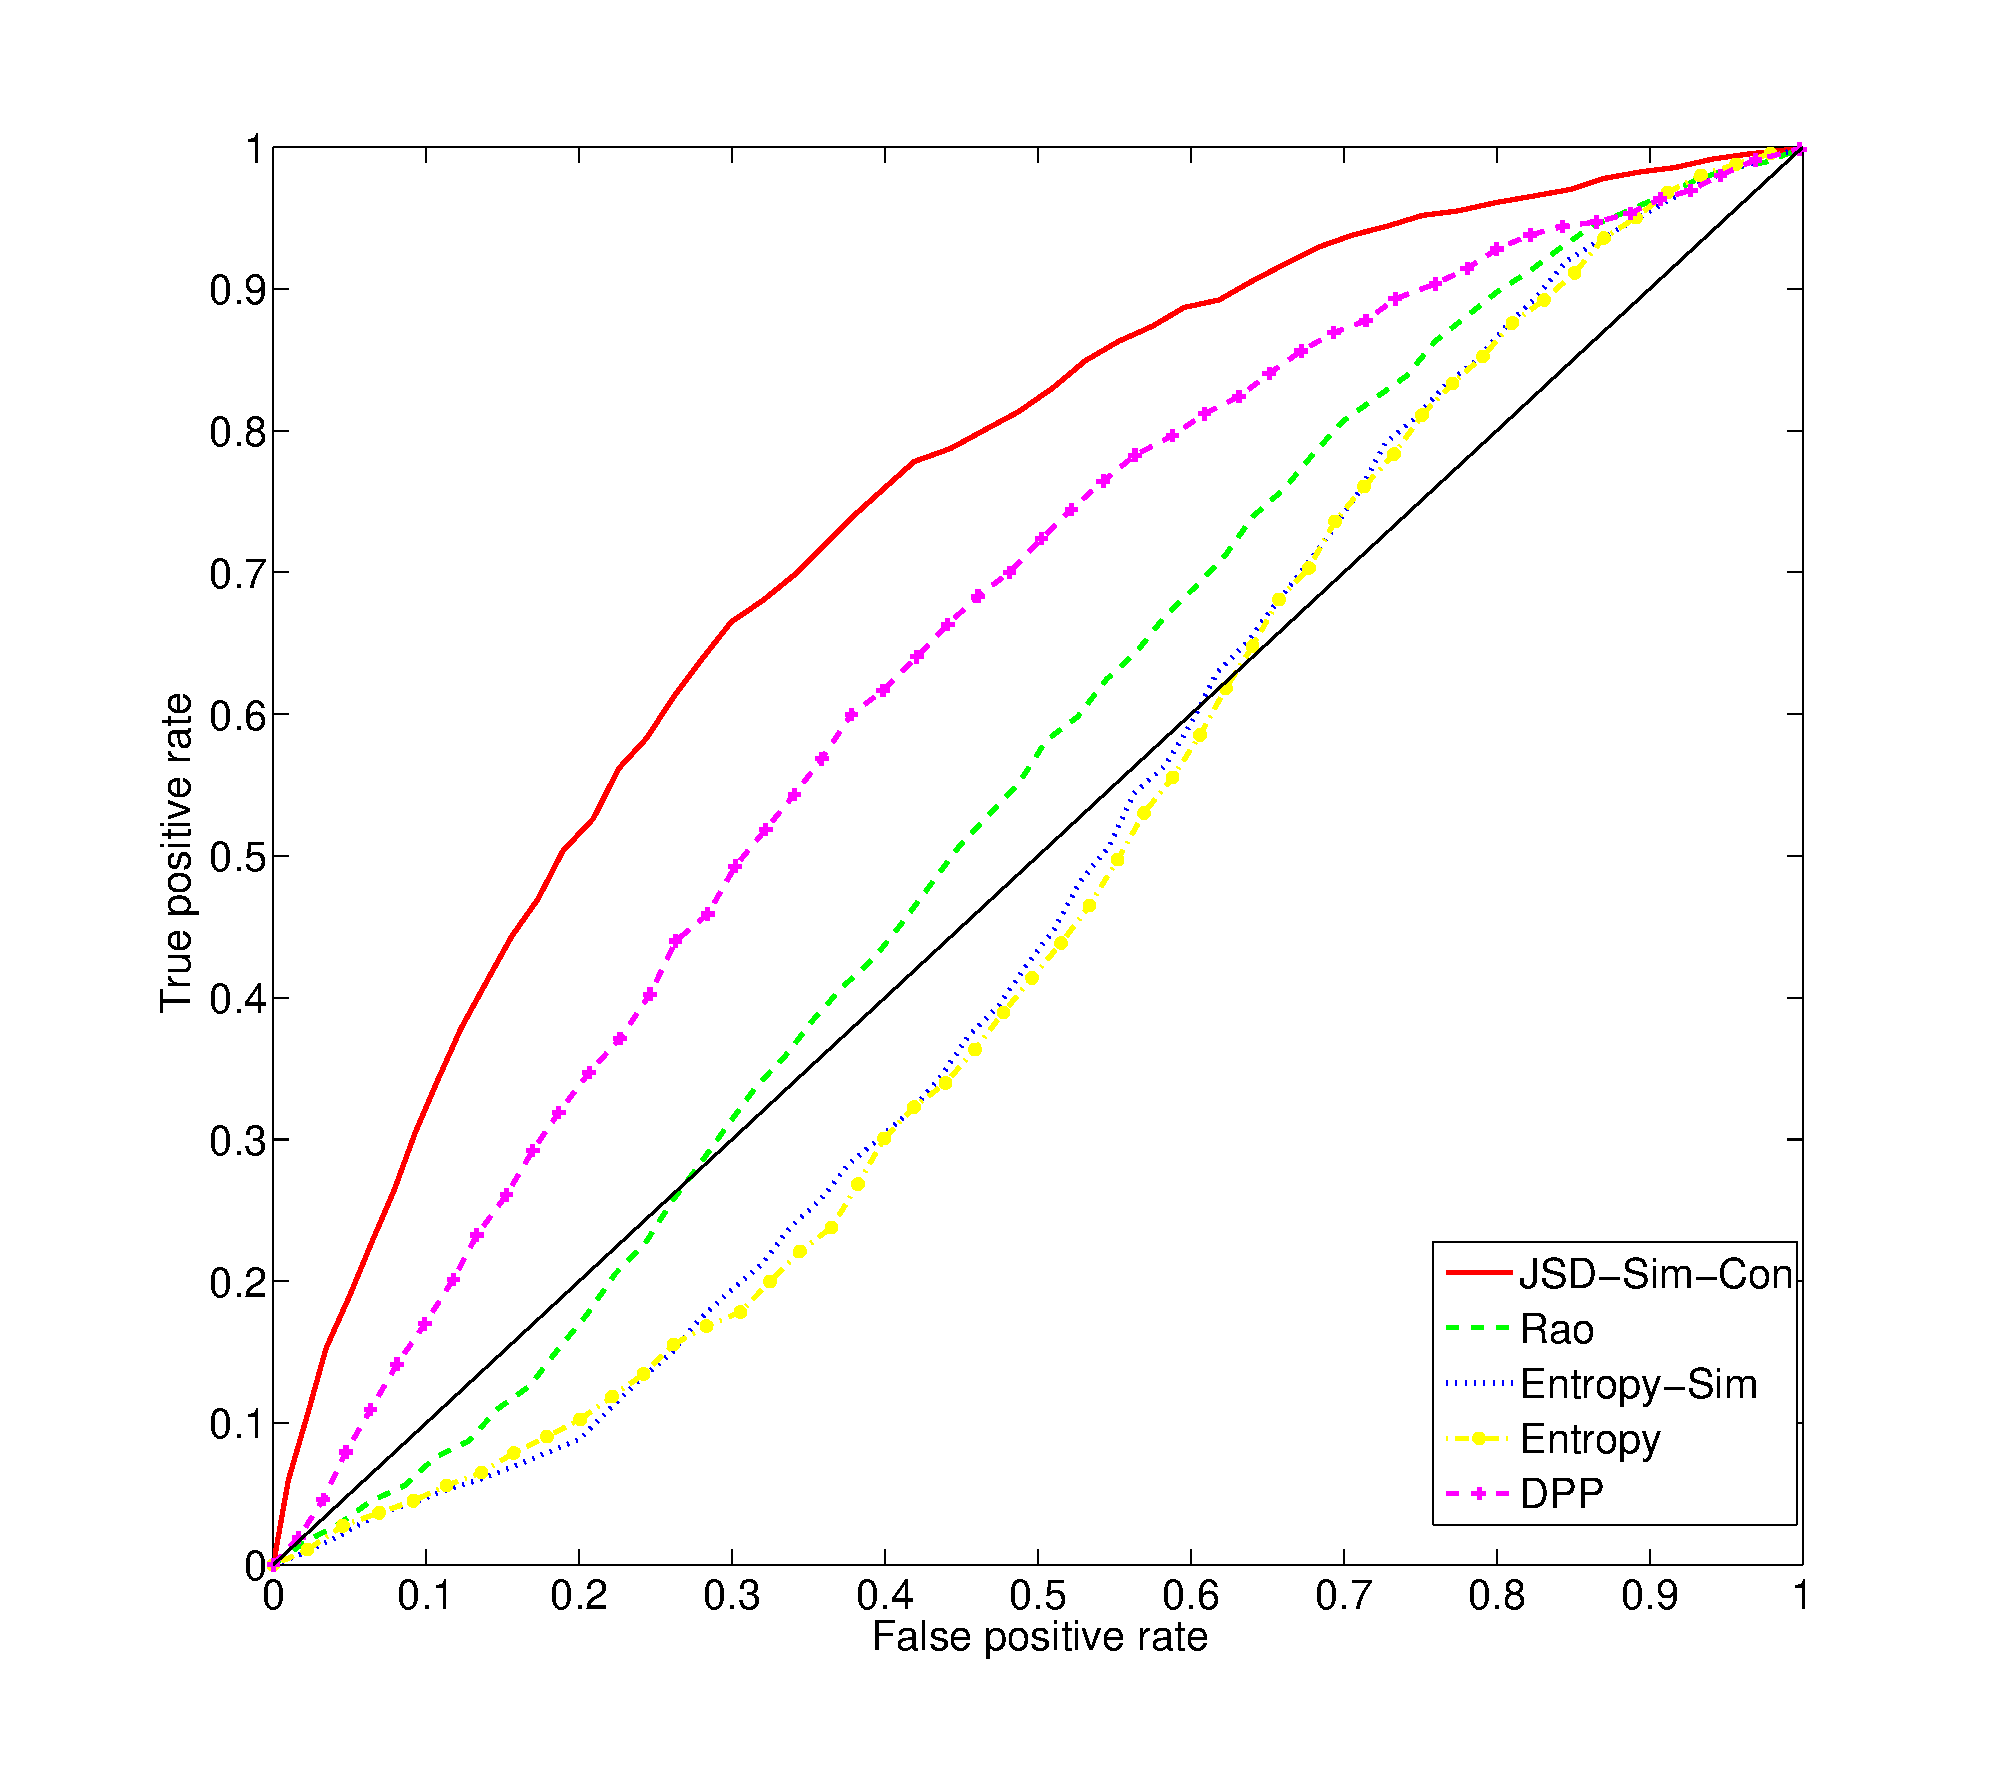
\includegraphics[width=36mm]{figures/phonecases-comparison-new.eps}
%                \caption{eBay (baseline)}
%                 \label{fig:phonecases-comparison}
%         \end{subfigure}%\qquad
%               ~ %add desired spacing between images, e. g. ~, \quad, \qquad, \hfill etc.
%           %(or a blank line to force the subfigure onto a new line)
%         \begin{subfigure}[b]{0.24\textwidth}
%                 \centering
%                 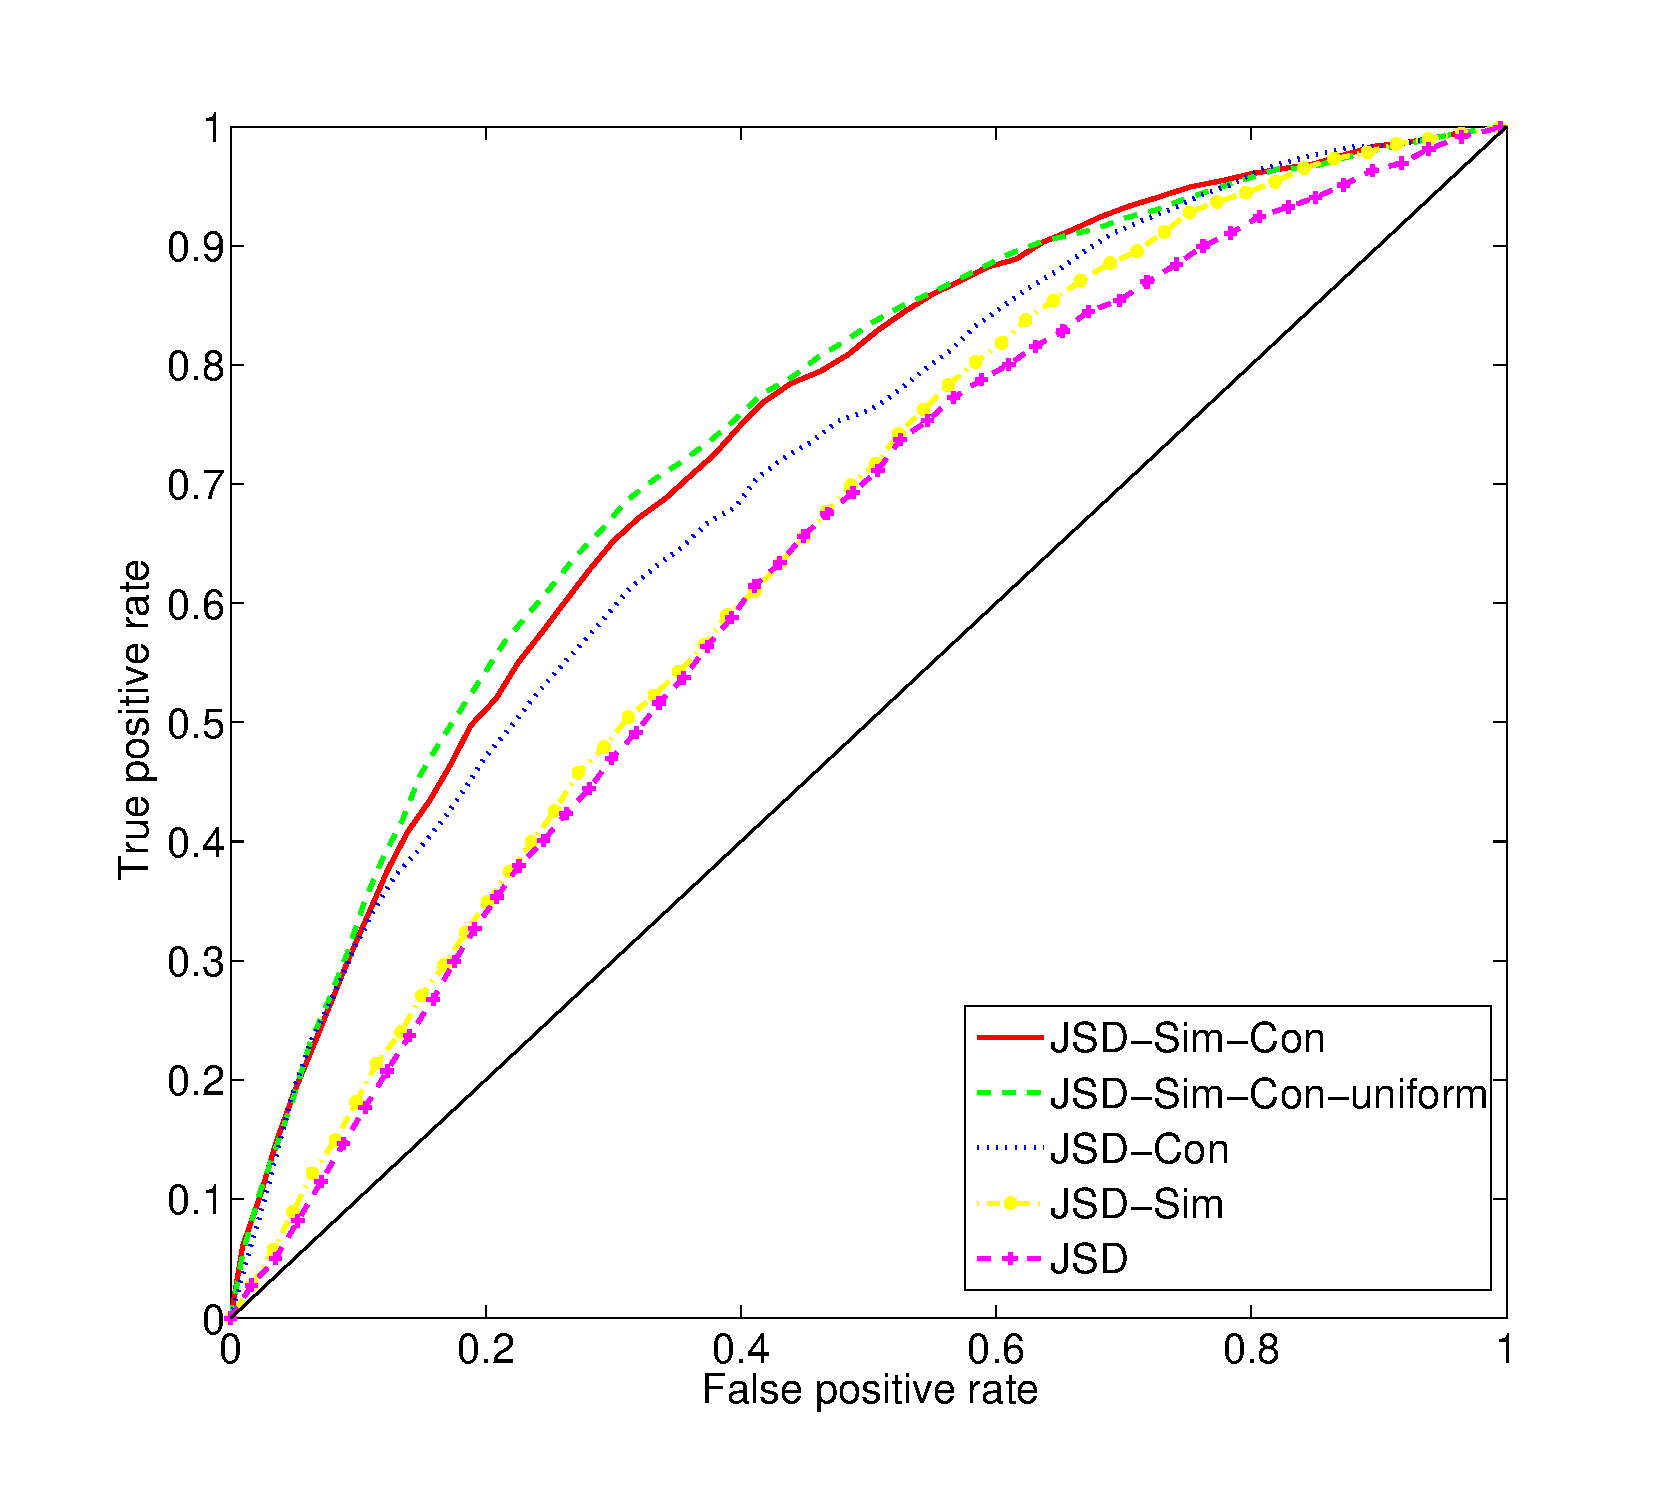
\includegraphics[width=36mm]{figures/phonecases-breakdown-new.eps}
%                 \caption{eBay (JSD)}
%                 \label{fig:phonecases-breakdown}
%         \end{subfigure}\nobreak
%               ~ %add desired spacing between images, e. g. ~, \quad, \qquad, \hfill etc.
%           %(or a blank line to force the subfigure onto a new line)
%         \begin{subfigure}[b]{0.24\textwidth}
%                 \centering
%                 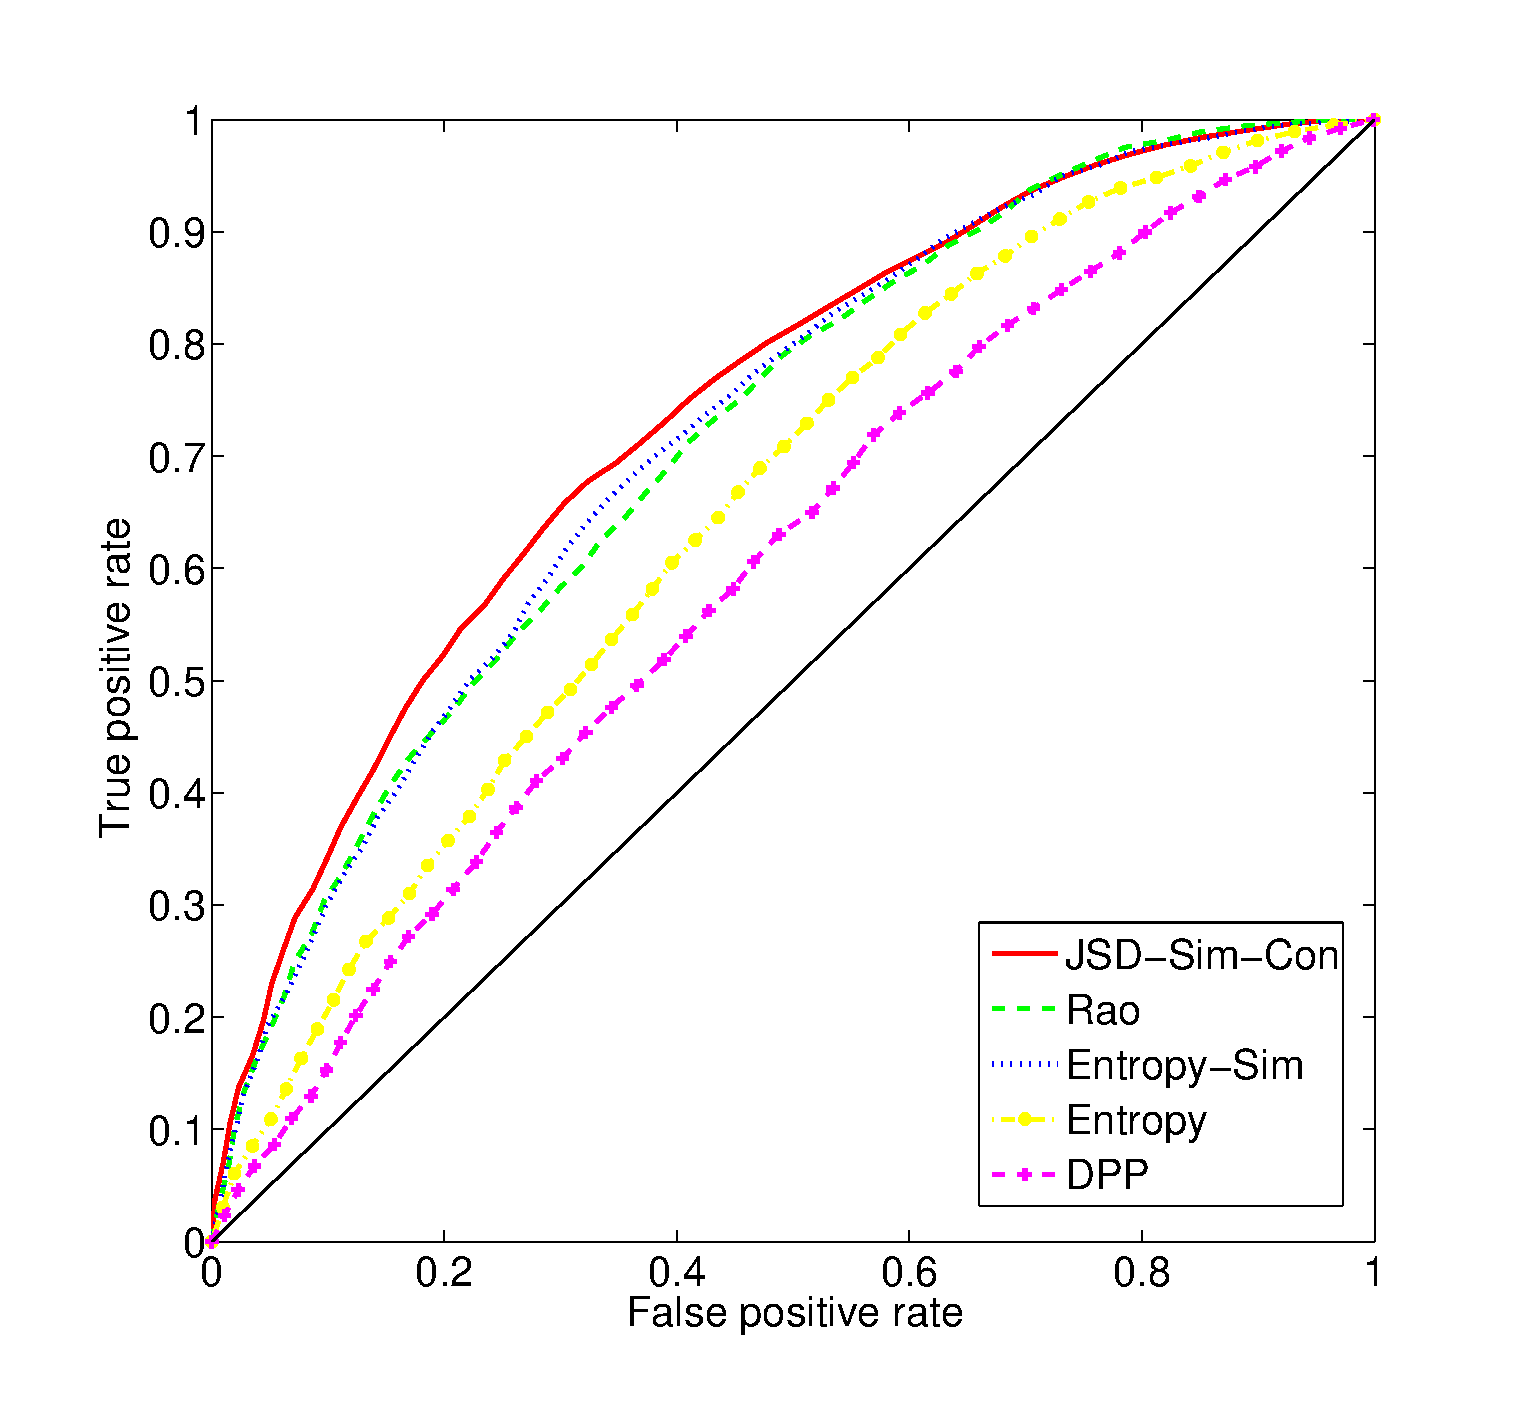
\includegraphics[width=36mm]{figures/nsf-comparison-new.eps}
%                 \caption{NSF (baseline)}
%                 \label{fig:nsf-comparison}
%         \end{subfigure}%\qquad
%         ~ %add desired spacing between images, e. g. ~, \quad, \qquad, \hfill etc.
%           %(or a blank line to force the subfigure onto a new line)
%         \begin{subfigure}[b]{0.24\textwidth}
%         	        \centering
%                 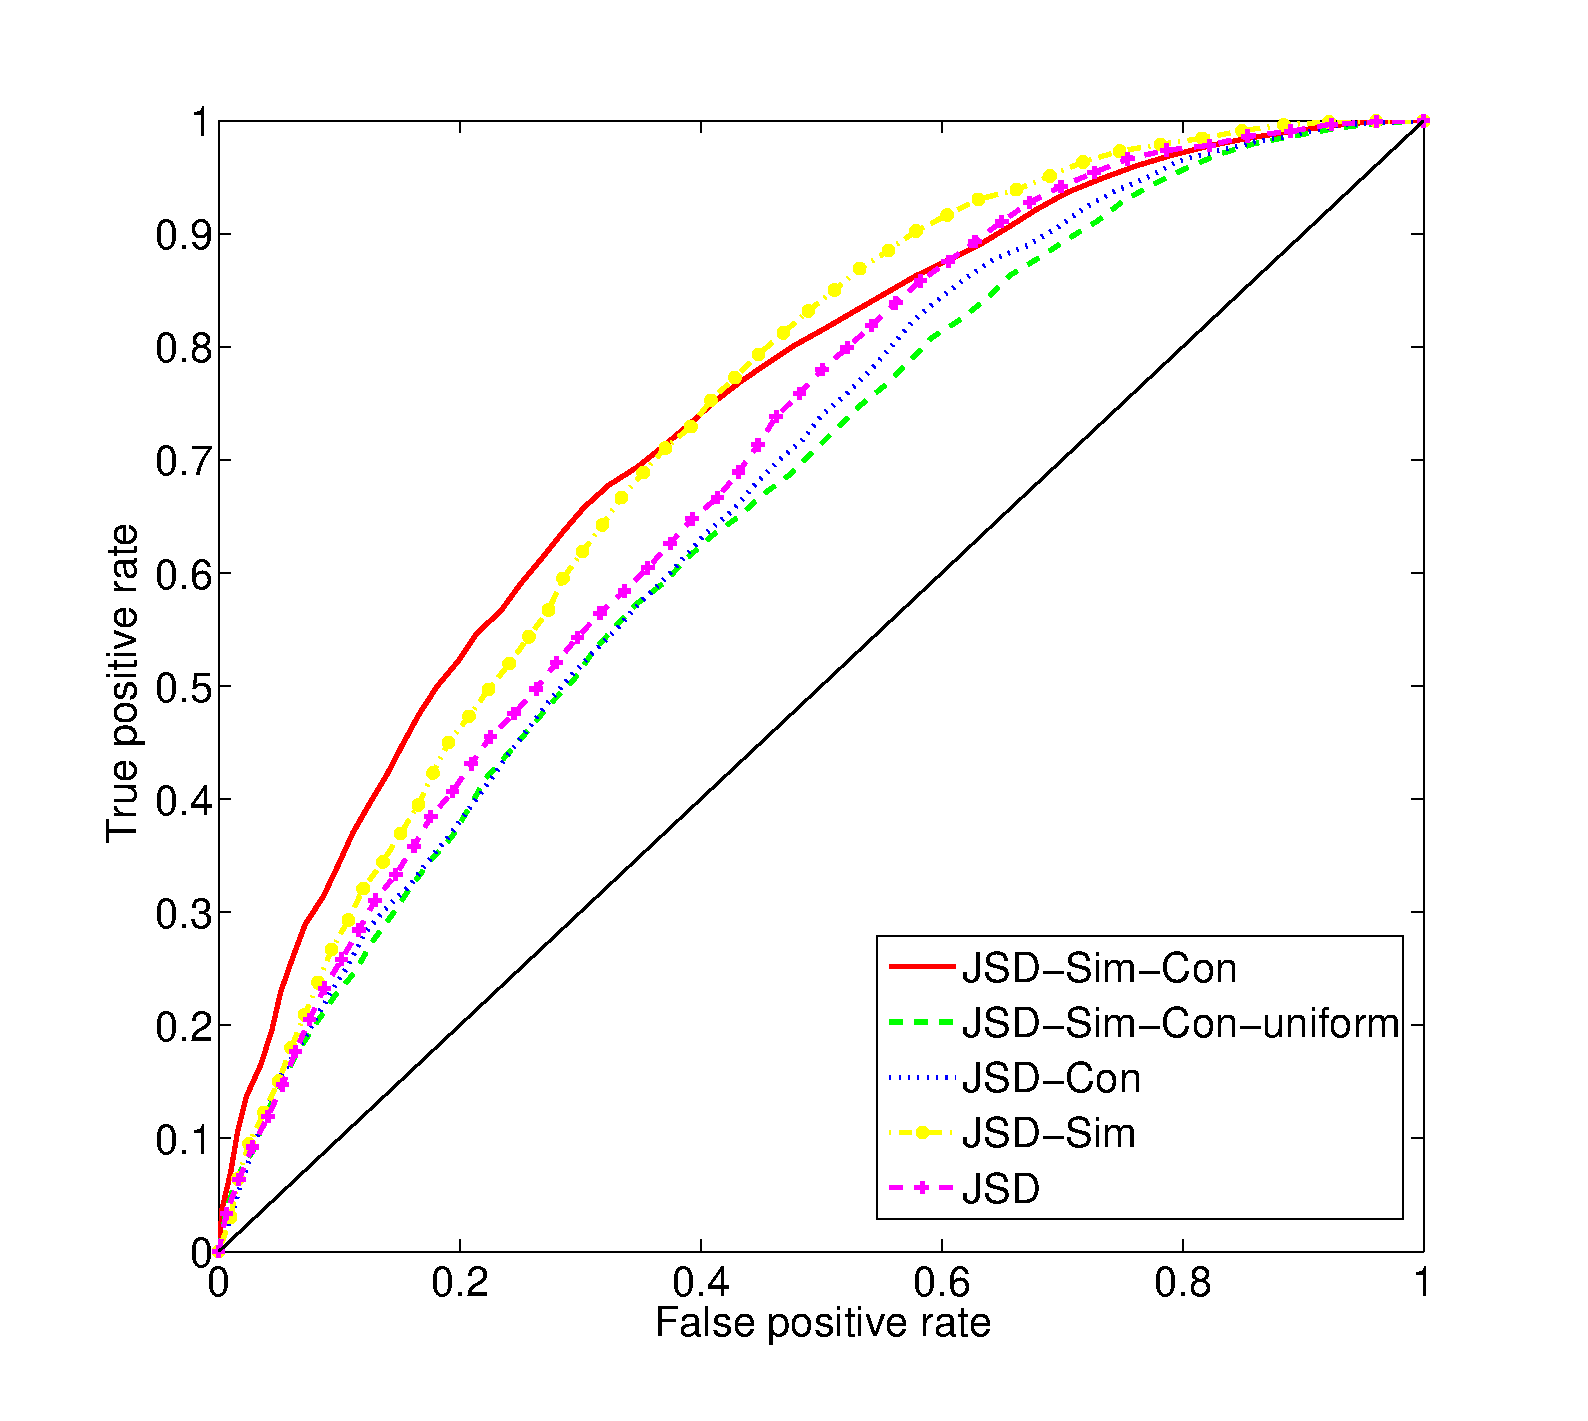
\includegraphics[width=36mm]{figures/nsf-breakdown-new.eps}
%                \caption{NSF (JSD)}
%                 \label{fig:nsf-breakdown}
%         \end{subfigure}
%        \caption{ROC curves presenting the results of experiments on
%          the eBay dataset (a,b) and NSF proposal dataset (c,d). The
%          comparison plots (a,c) show the results for our approach (JSD-Sim-Con)
%          against other methods, while the plots (b,d)
%          show different variations of our approach. }\label{fig:roc-curves}
% \end{figure}


\subsection{Results}
\label{sec:results}


\begin{table*}[t]
\begin{center}
\begin{tabular}{CC}
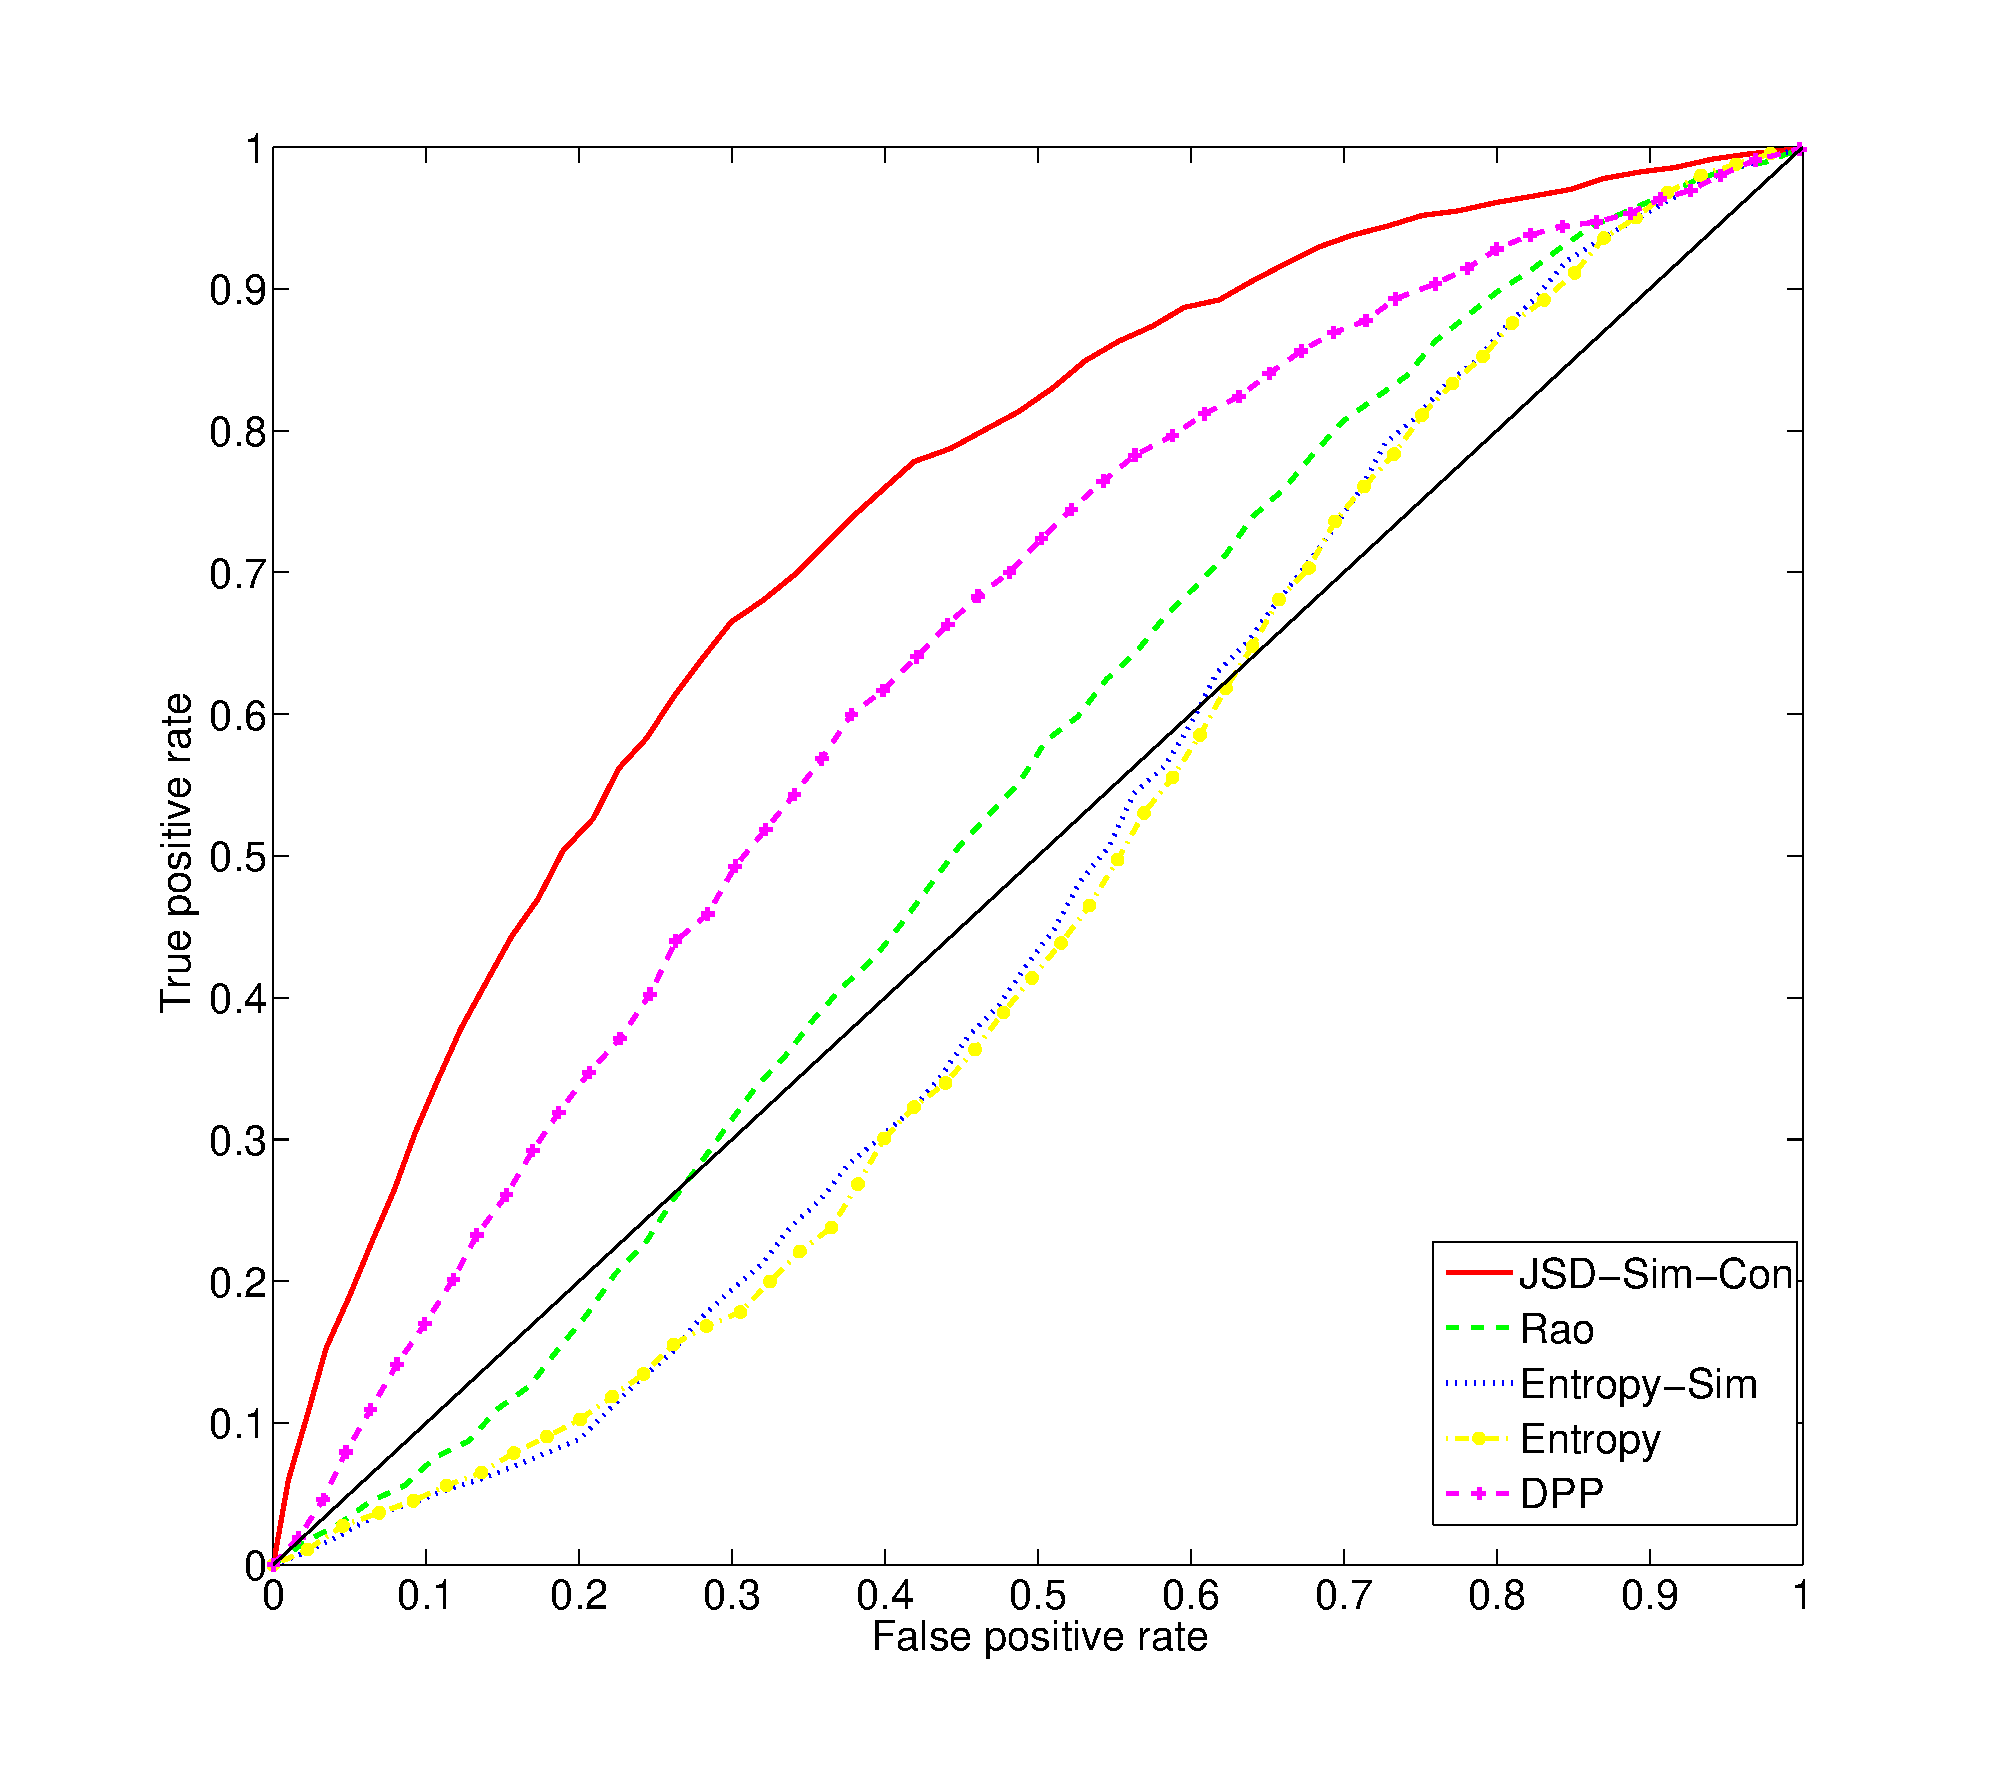
\includegraphics[height=6.5cm]{figures/phonecases-comparison-new.eps}&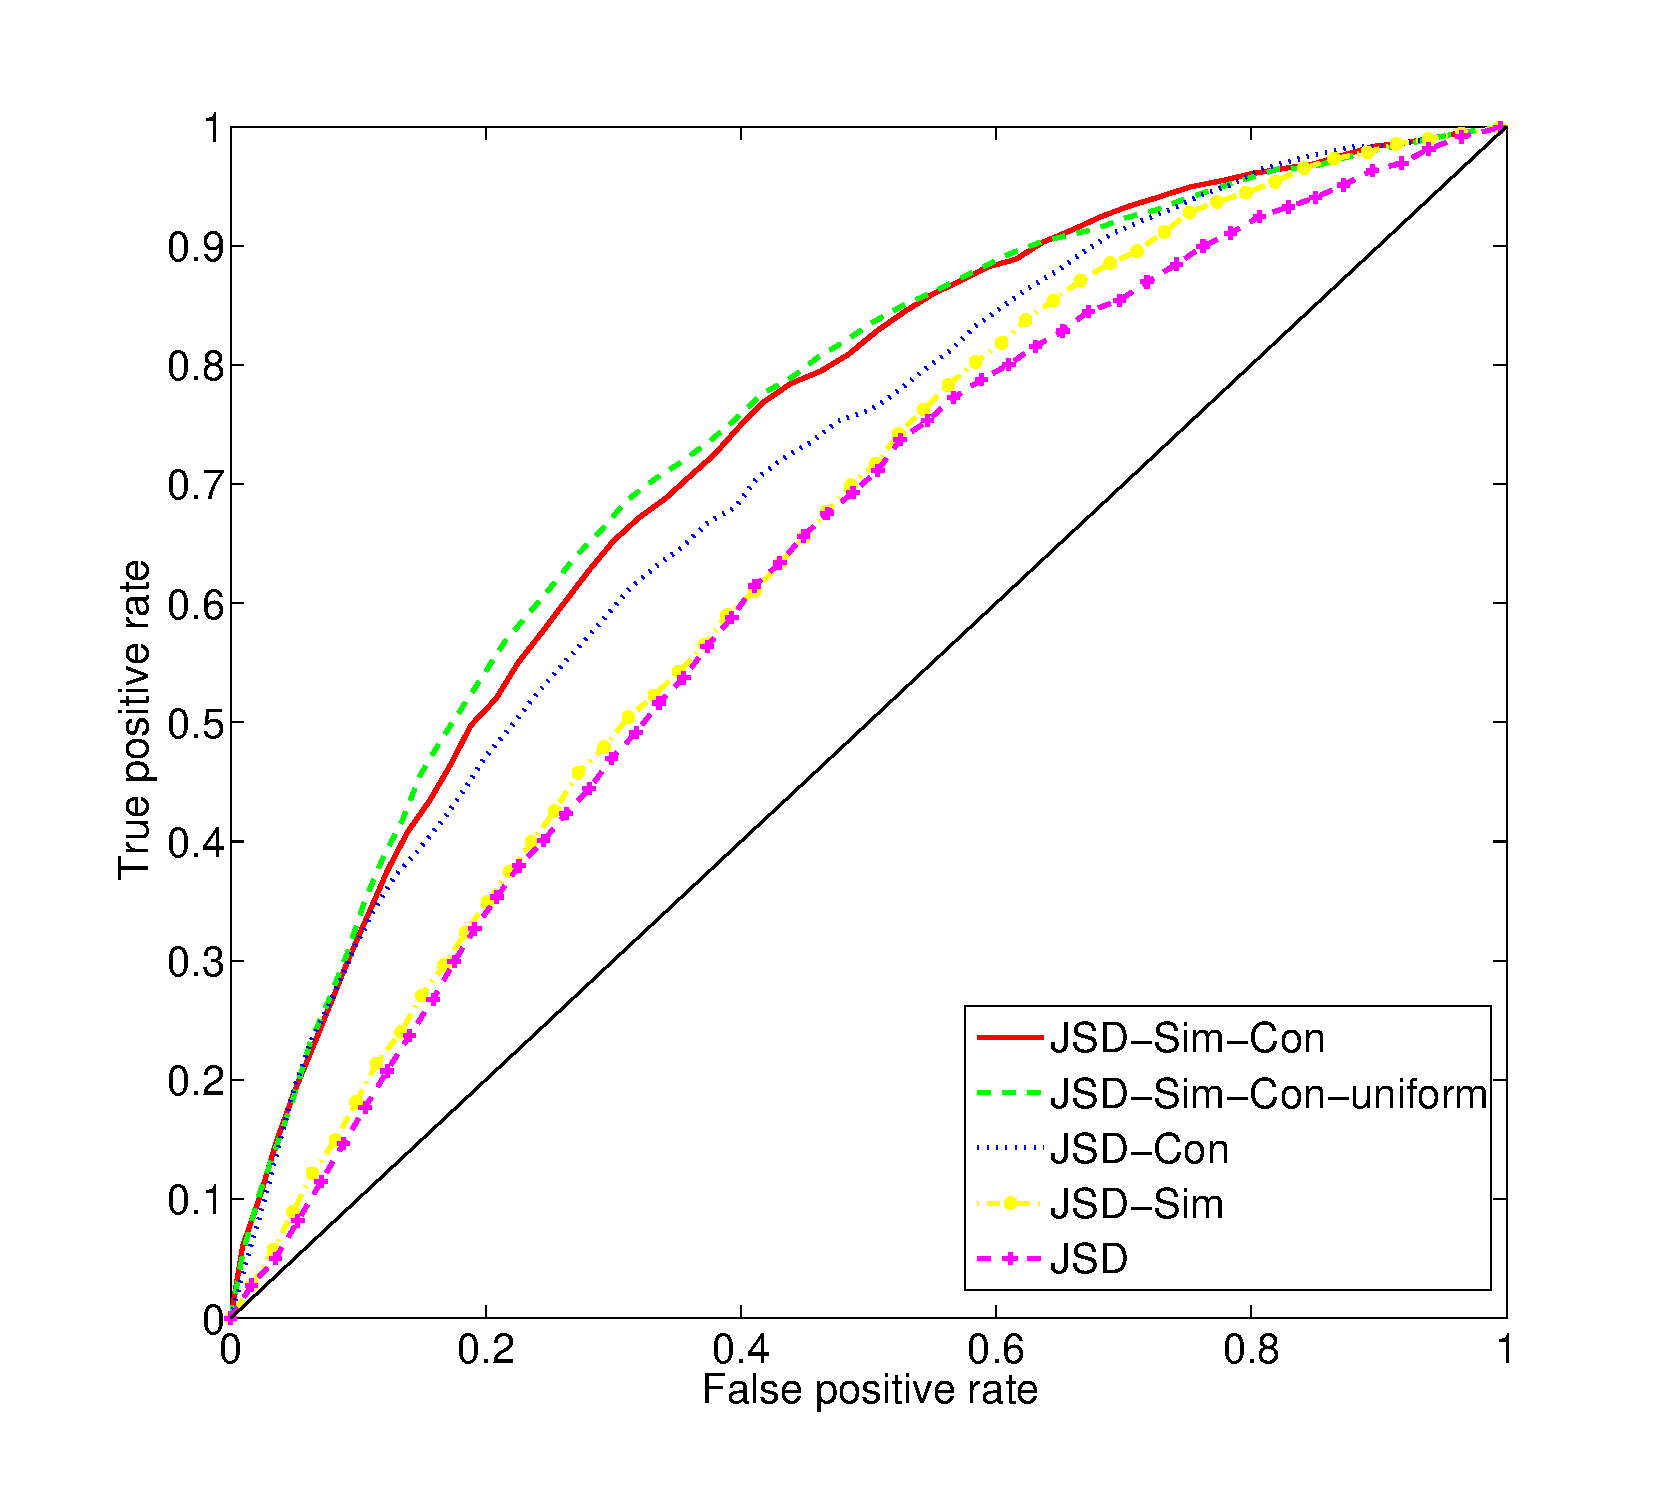
\includegraphics[height=6.5cm]{figures/phonecases-breakdown-new.eps}\\
(a) & (b)\\
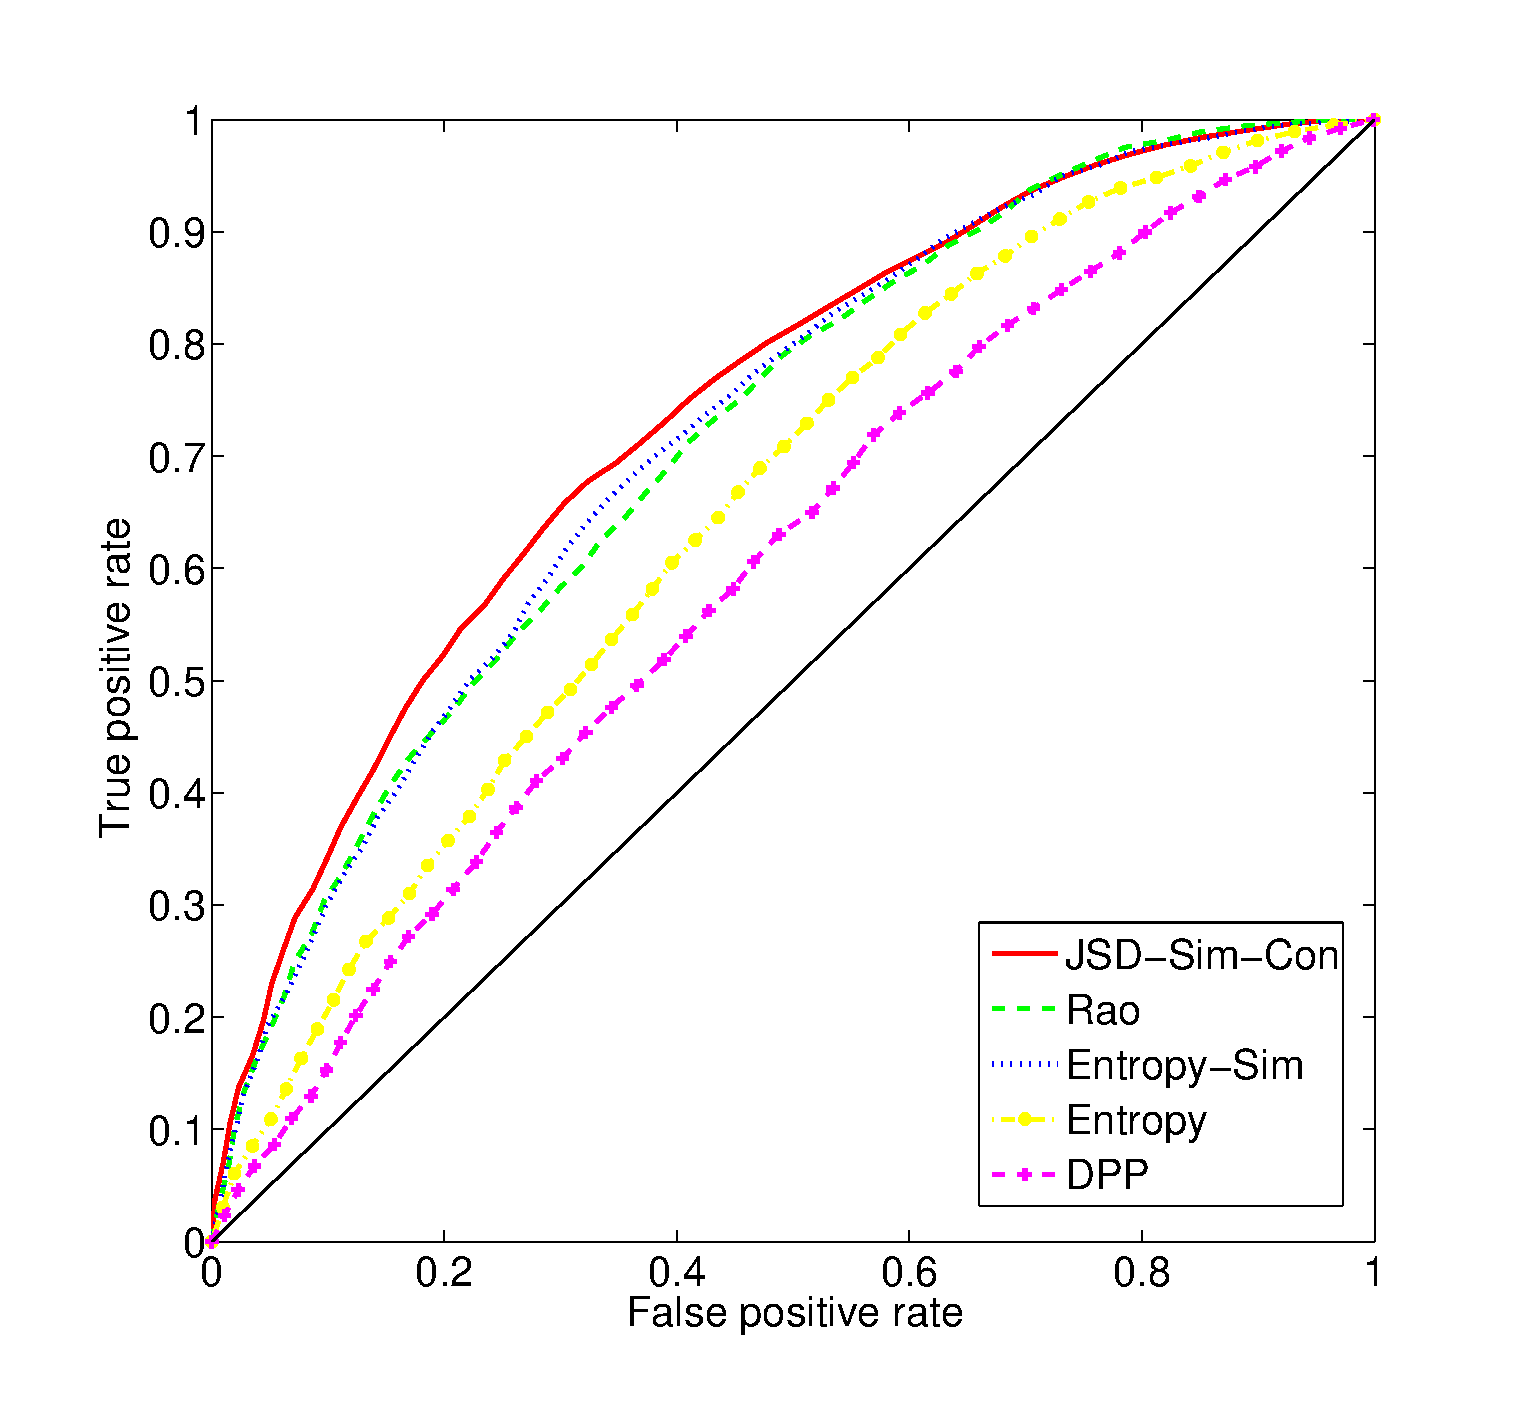
\includegraphics[height=6.5cm]{figures/nsf-comparison-new.eps}&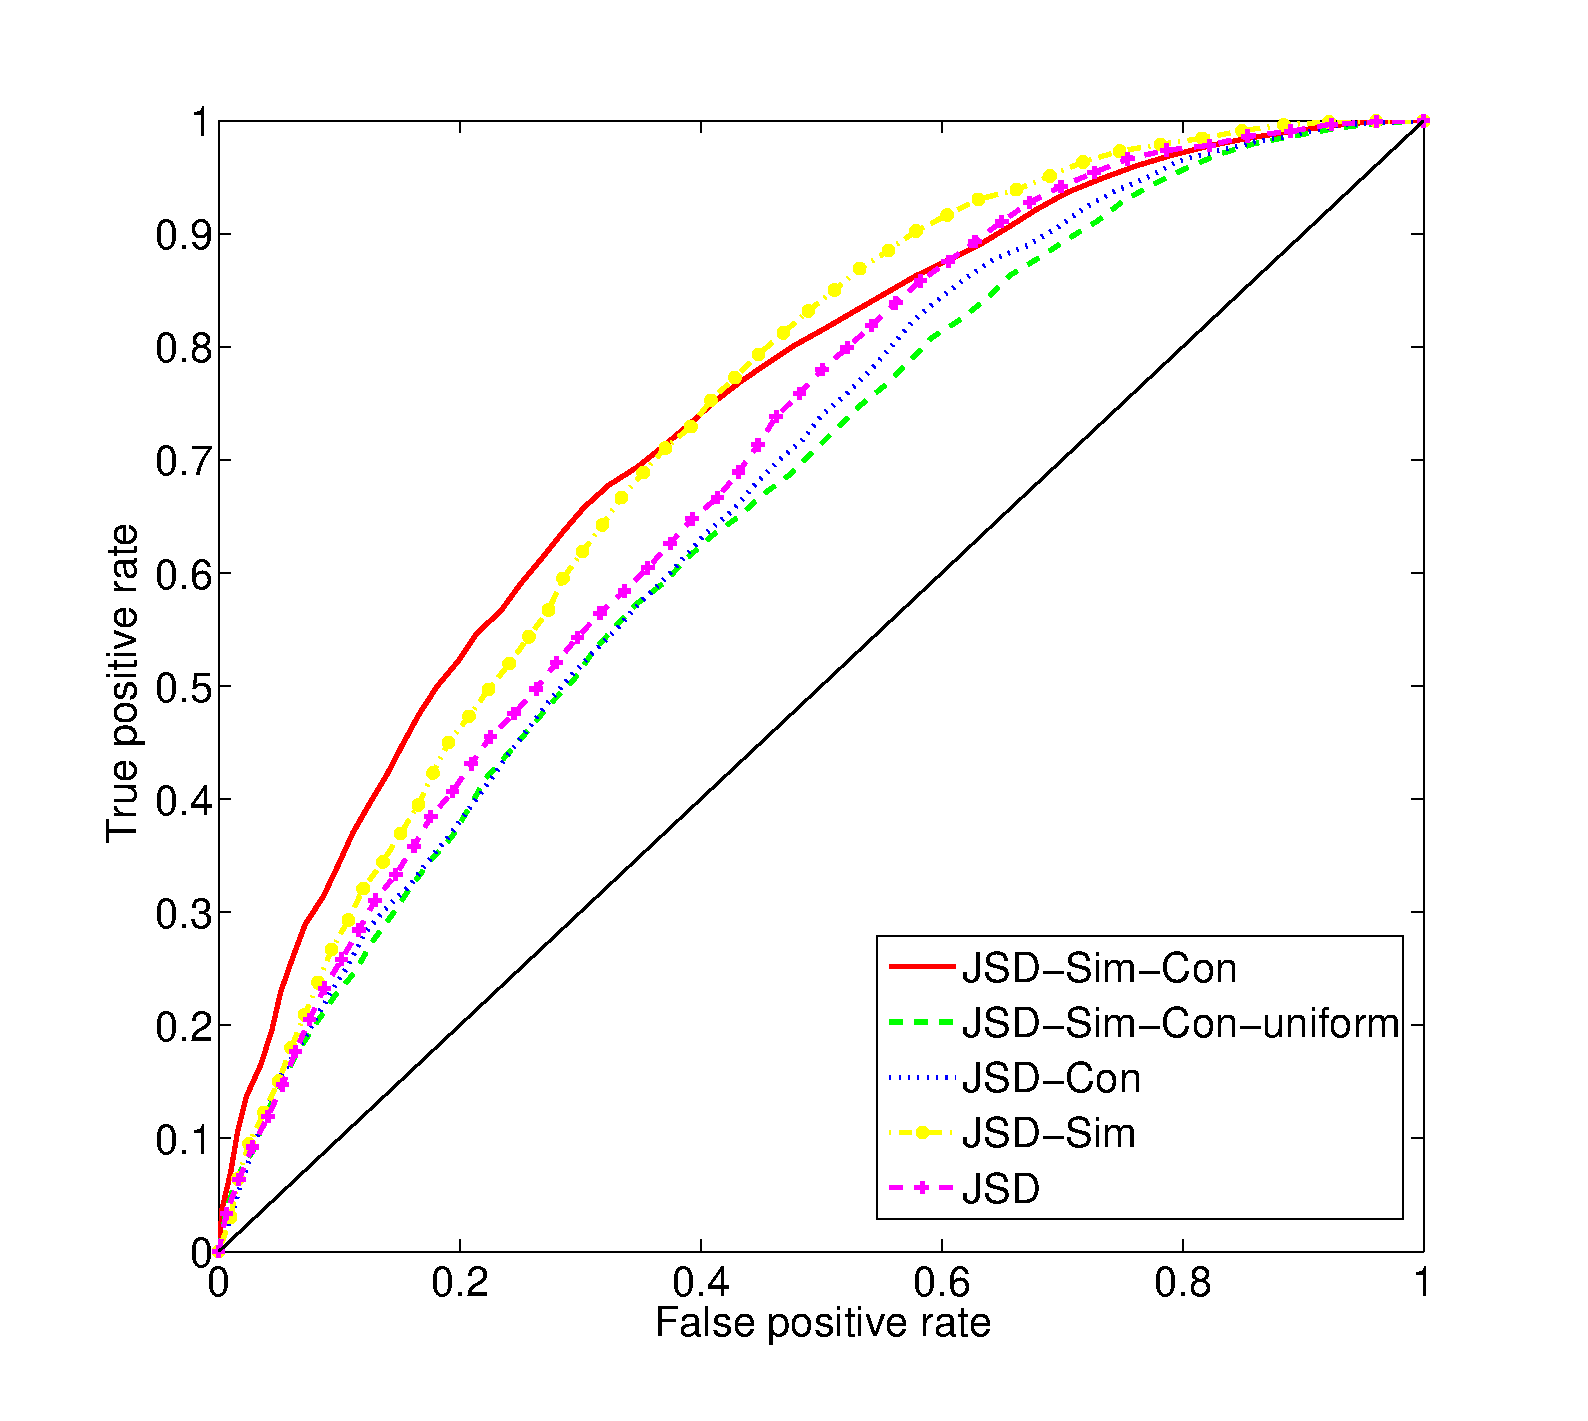
\includegraphics[height=6.5cm]{figures/nsf-breakdown-new.eps}\\
(c) & (d)\\
\end{tabular}
\end{center}
\caption{ROC curves presenting the results of experiments on
the eBay dataset (a,b) and NSF proposal dataset (c,d). The
comparison plots (a,c) show the results for our approach (JSD-Sim-Con)
against other methods, while the plots (b,d)
show different variations of our approach. }
\label{fig:roc-curves}
\end{table*}


In either case it can be observed
that our diversity metric outperforms the other baselines with an AUC
around $0.73$. Moreover, for the {\em eBay} dataset the other measures
give poor results. This can be explained as follows: since the
text snippets are short, the LDA may yield a poor topic inference for such short text and as a result all measures using topic inference would perform poorly. Figures~\ref{fig:phonecases-breakdown} and \ref{fig:nsf-breakdown} show the gains we obtain by applying topic similarity and context conditioning techniques (steps 4 and 5) that we discussed in Section~\ref{sec:topic-diversity}. However, their degree of effects is different for each
dataset.  

\begin{table*}[t]
\label{tab:classification-results}
%\vspace{-4mm}
\begin{center}
\begin{tabular}{|l|c|c|c|c|}
\hline
&Precision & Recall & F1 & Accuracy
\\ \hline 
JSD Features         &$\mathbf{0.714}\pm 0.015$&$0.597\pm 0.016$&$0.650\pm
0.014$& $\mathbf{0.8828}\pm 0.0045$\\
RAE             &$0.676\pm 0.005$&$\mathbf{0.666}\pm 0.030$&$\mathbf{0.671}\pm
0.013$&$0.8809\pm 0.0020$ \\
SVD Features             &$0.676\pm 0.008$&$0.633\pm 0.017$&$0.654\pm
0.010$&$0.8778\pm 0.0027$\\
\hline
\end{tabular}
\caption{Classification results for the eBay dataset.}
\end{center}
\end{table*}

In the second set of results, we used the unnormalized vector of mixture topic
distribution (described in Definition~\ref{mixture}) computed over
{\em eBay} product titles in a supervised classification
setting. Table~\ref{tab:classification-results} shows
the performance of the SVM classifier using our proposed mixture topic
distribution as features and compares it to two different baselines, namely, SVM using
{\em Latent Semantic Indexing (LSI)} features (by forming a
document-term matrix and performing SVD), and a deep learning approach
using the {\em recursive auto-encoders (RAE)} framework described
in~\cite{Socher:2011:SRA:2145432.2145450}. These results are averaged
over five different cross-validation splits using $0.6$ for training
and $0.4$ for testing. Our proposed approach shows a higher precision
and a marginally higher accuracy compared to the baselines.
